%--------------------------------------------------------------------------
%	PACKAGES AND OTHER DOCUMENT CONFIGURATIONS
%--------------------------------------------------------------------------
\documentclass[11pt,a4paper]{article}
\usepackage[utf8]{inputenc}
\usepackage[english]{babel}
\usepackage[T1]{fontenc}
\usepackage{amsmath}
\usepackage{mathtools}
\usepackage{amsfonts}
\usepackage{amssymb}
\usepackage{pifont}% http://ctan.org/pkg/pifont
\usepackage{graphicx}
\usepackage{epstopdf}
\usepackage{lmodern}
\usepackage[left=3cm,right=3cm,top=2.5cm,bottom=2.5cm]{geometry}

\usepackage{fancyhdr} % Required for custom headers
\usepackage{lastpage} % Required to determine the last page for the footer
\usepackage{extramarks} % Required for headers and footers
\usepackage[usenames,dvipsnames]{color} % Required for custom colors
\usepackage{graphicx} % Required to insert images
\usepackage{caption}
\usepackage{subcaption}
\usepackage{listings} % Required for insertion of code
%\usepackage{courier} % Required for the courier font
\usepackage{verbatim}
\usepackage{multirow}
\usepackage{eurosym}
\usepackage{url}
\usepackage{hyperref}
\usepackage{color}
\usepackage[outline]{contour}
 \contourlength{.5pt}
\usepackage[noadjust]{cite}
\usepackage{tabularx}

\usepackage{enumerate}
%\usepackage{todonotes}
%\usepackage{relsize}

\usepackage{tikz}
\usetikzlibrary{matrix}

\setlength\parindent{0pt} % Removes all indentation from paragraphs
\setlength{\parskip}{10pt plus 1pt minus 1pt}

%\definecolor{bleu}{HTML}{0000FF}
%\definecolor{jaune}{HTML}{EDB601}
%\definecolor{vert}{HTML}{008E45}
%\definecolor{rouge}{HTML}{FF0000}

%\renewcommand\thesection{\Roman{section}}

\begin{document}
	
%--------------------------------------------------------------------------
%	TITLE PAGE
%--------------------------------------------------------------------------
\begin{center}
{\bfseries
Linköping University\\
TDDD17 Information Security, Second Course\\

Lab 1: Authentication with OpenID\\
Lab assistant: Ulf Kargén\\[10pt]}

Guillaume Lambert (guila302) and Lena Peschke (lenpe782)\\
version 1, 15-01-27
\end{center}

\hrulefill

%--------------------------------------------------------------------------
%	CONTENT
%--------------------------------------------------------------------------

\section*{Our own authentication method}
\subsection*{Design of an authentication method}
\paragraph{Description}
% design choices
% -> combination of matrix positions, colours, (letters?)
% how it works

Our authentication method is challenge-response. It is based on a choice of matrix positions, colors and a password made at the registration.
These choices determine the answer to the challenges that are sent by the server to the user.

More concretely the challenge consists of a randomly generated $3\times3$-matrix in which each of the 9 positions may contain a different letter and color.
The answer the user has to provide is made of the letters that fit his choices by either being in the
right position inside the matrix, of the right color, or simply a letter contained in the password. The user thus has to identify the components that overlap with his personal secret.

If no letters fit at least one of the chosen characteristics the entire password has to be entered.

The parameters among which the user has to choose are:
\begin{itemize}
\item 3 to 7 matrix positions (among 9)
\item 2 to 4 colours among 6 (black, white, red, blue, green, violet)
\item a password of maximum 12 letters but with at least 4 different letters. Case is not considered.
\end{itemize}

\textit{Example:} A user chooses the following scheme.
\begin{itemize}
\item matrix positions: $(1,3) (2,3) (3,2) (3,3)$
\item colours: \textcolor{blue}{blue} \textcolor{green}{green} \textcolor{violet}{violet}
\item password: \texttt{password}
\end{itemize}

When presented with a randomly generated challenge as presented in Figure~\ref{fig:ex1}, the user has to select the squares containing A, I, and X. His answer will be any permutation of \texttt{aix}.
\begin{figure}
\centering
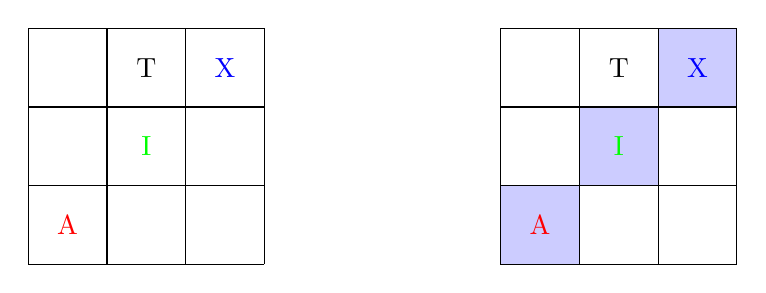
\begin{tikzpicture}
\draw[step=1cm,color=black,thin] (0,0) grid (3,3);
\node[red] at (0.5,0.5) {A};
\node[black] at (1.5,2.5) {T};
\node[green] at (1.5,1.5) {I};
\node[blue] at (2.5,2.5) {X};

\draw[step=1cm,color=black,thin] (6,0) grid (9,3);
\filldraw[fill=blue!20!white, draw=black] (6,0) rectangle (7,1);
\filldraw[fill=blue!20!white, draw=black] (7,1) rectangle (8,2);
\filldraw[fill=blue!20!white, draw=black] (8,2) rectangle (9,3);
\node[red] at (6.5,0.5) {A};
\node[black] at (7.5,2.5) {T};
\node[green] at (7.5,1.5) {I};
\node[blue] at (8.5,2.5) {X};
\end{tikzpicture}
\caption{Example of a challenge-response. The left matrix is the challenge and the right the response, where the blue squares are the ones selected by the user.}
\label{fig:ex1}
\end{figure}

\paragraph{Risk analysis}
% security conclusions
% compare to passwords
% weaknesses + mitigate them

\paragraph{Use-case diagram}

\paragraph{Sequence diagram}

\subsection*{Implementation of an authentication method}
\paragraph{Overview}
% how to implement

\paragraph{Database}
\paragraph{User interface}
\paragraph{HTML and CSS}
\paragraph{Servlets}
\paragraph{OpenIDA}

\end{document}
